\section{1174083 - Bakti Qilan Mufid}
Chapter 7 - CNN
\subsection{Teori}
\subsubsection{Jelaskan kenapa file teks harus dilakukan tokenizer. dilengkapi dengan ilustrasi atau gambar.}
\hfill\\
Karena untuk memudahkan mesin memahami maksud dari apa yang usr inginkan. Dalam teks file, kata disebut token, dan proses vektorisasi dari bentuk kata kedalam bentuk token tersebut disebut tokenizer dan tokenizer akan merubah sebuah teks menjadi simbol, kata, ataupun biner dan bentuk lainya kedalam token. Untuk ilustrasinya bisa seperti berikut, terdapat sebuah kalimat a=yang akan dilakukan tokenizer kalimatnya: "jangan panggil aku anak kecil paman" maka ketika dilakukan tokenizer hasilnya akan menjadi ['jangan','panggil','aku','anak','kecil','paman'].

\subsubsection{Jelaskan konsep dasar K-Fold Cross Validation pada dataset komentar Youtube pada kode listing 7.1 dilengkapi dengan ilustrasi atau gambar.}
\hfill\\
\lstinputlisting[firstline=8, lastline=9, caption={K-fold Cross Validation},captionpos=b]{src/1174083/src7/teori.py}

Konsep sederhana dari K-Fold Cross Validation pada code tesebut ialah terdapat kfold yang bertujuan untuk melakukan split data menjadi 5 bagian dari dataset komentar Youtube tersebut. Sehingga dari setiap data yang sudah dibagi tersebut akan menghasilkan presentase dari setiap bagiannya, untuk menghasilkan hasil akhir dengan presentase yang cukup baik. Untuk ilustrasi, lihat gambar berikut: 

\begin{figure}[H]
	\centering
	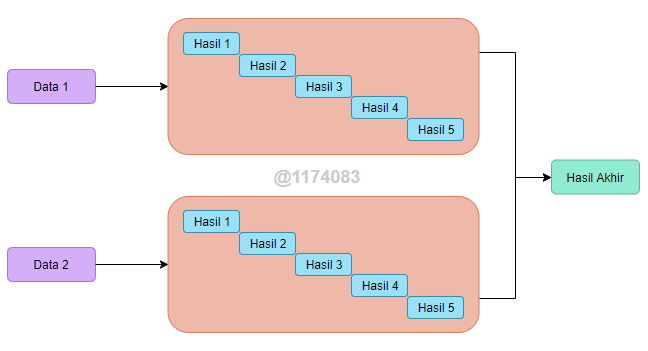
\includegraphics[width=8cm]{figures/1174083/figures7/1.png}
	\caption{gambaran penjelasan no. 2}
\end{figure}

\subsubsection{Jelaskan apa maksudnya kode program \textit{for train, test in splits}. dilengkapi dengan gambar atau ilustrasi}
\hfill\\
Untuk penjelasan nya yaitu For train berfungsi untuk membagi data tersebut menjadi data training. Sedangkan test in splits berfungsi untuk menguji apakah dataset tersebut sudah dibagi menjadi beberapa bagian atau masih menumpuk.
\begin{figure}[H]
	\centering
	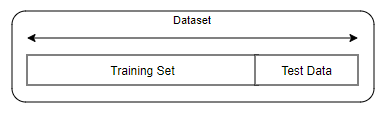
\includegraphics[width=8cm]{figures/1174083/figures7/2.png}
	\caption{gambaran penjelasan no. 3}
\end{figure}

\subsubsection{jelaskan maksudnya kode program}
Maksudnya yaitu mengambil data pada kolom atau index CONTENT yang merupakan bagian dari train\_idx dan test\_idx. Ilustrasinya, ketika data telah diubah menjadi train dan test maka kita dapat memilihnya untuk ditampilkan pada kolom yang diinginkan. untuk ilustrasinya ada pada kode berikut:
\lstinputlisting[firstline=12, lastline=21]{src/1174083/src7/teori.py}
\begin{figure}[H]
	\centering
	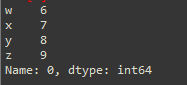
\includegraphics[width=10cm]{figures/1174083/figures7/3.png}
	\caption{gambaran penjelasan no. 4}
\end{figure}

\subsubsection{Jelaskan apa maksud dari fungsi dilengkapi dengan ilustrasi atau gambar}
\hfill\\
Fungsi tokenizer ini berfungsi untuk melakukan vektorisasi data kedalam bentuk token sebanyak 2000 kata. Dan selanjutnya akan melakukan fit tokenizer hanya untuk data training saja tidak dengan data testingnya. Untuk ilustrasi lihat gambar berikut: 
\begin{figure}[H]
	\centering
	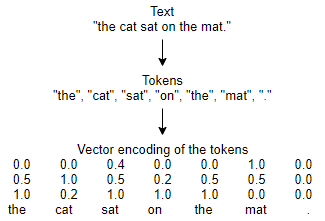
\includegraphics[width=8cm]{figures/1174083/figures7/4.png}
	\caption{gambaran penjelasan no. 5}
\end{figure}

\subsubsection{Jelaskan apa maksud dari dilengkapi dengan ilustrasi kode dan atau gambar}
\hfill\\
Maksudnya yaitu untuk variabel d\_train\_inputs akan melakukan tokenizer dari bentuk teks ke matrix dari data train\_content dengan mode matriksnya yaitu tfidf begitu juga dengan variabel d\_test\_inputs untuk data test.
\begin{figure}[H]
	\centering
	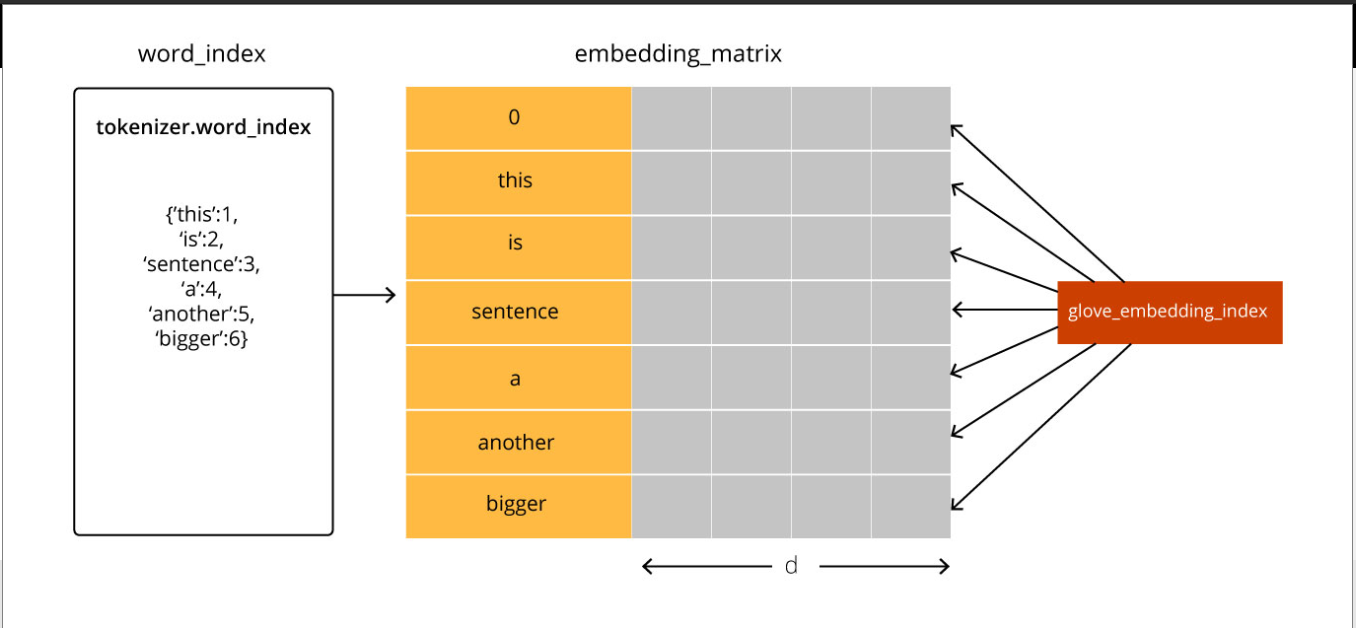
\includegraphics[width=10cm]{figures/1174083/figures7/5.png}
	\caption{gambaran penjelasan no. 6}
\end{figure}

\subsubsection{Jelaskan apa maksud dari fungsi dilengkapi dengan ilustrasi atau gambar}
\hfill\\
Fungsi tersebut akan membagi matrix tfidf tadi dengan np.amax yaitu mengembalikan maksimum array atau maksimum sepanjang sumbu. Jika sumbu tidak ada, hasilnya adalah nilai skalar. Jika sumbu diberikan, hasilnya adalah array dimensi a.ndim - 1. Yang hasilnya akan dimasukan kedalam variabel d\_train\_inputs untuk data train dan d\_test\_inputs untuk data\_test dengan nominal absolut atau tanpa ada bilangan negatif dan koma.
\begin{figure}[H]
	\centering
	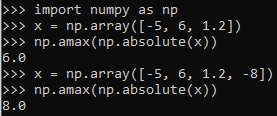
\includegraphics[width=10cm]{figures/1174083/figures7/6.png}
	\caption{gambaran penjelasan no. 7}
\end{figure}

\subsubsection{Jelaskan apa maksud dari  dilengkapi dengan ilustrasi atau gambar}
\hfill\\
Dalam variabel d\_train\_output dan d\_test\_outputs akan dilakukan one-hot-encoding, dimana np\_utils akan mengubah vektor dengan bentuk integer ke matriks kelas biner untuk kolom CLASS dimana nantinya hanya akan ada dua pilihan yaitu 1 atau 0. 1 untuk spam 0 untuk non spam atau sebaliknya.
\begin{figure}[H]
	\centering
	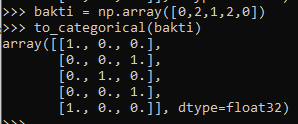
\includegraphics[width=10cm]{figures/1174083/figures7/7.png}
	\caption{gambaran penjelasan no. 8}
\end{figure}

\subsubsection{Jelaskan apa maksud dari fungsi di listing 7.2. Gambar Neural Networknya dari model kode tersebut}
\hfill\\
\lstinputlisting[firstline=24, lastline=29, caption={model Neural Network},captionpos=b]{src/1174083/src7/teori.py}
Penjelasannya sebagai berikut :
\begin{itemize}
\item Melakukan pemodelan Sequential
\item Layer pertama dense dari 512 neuron untuk inputan dengan inputan tadi yang sudah dijadikan matriks sebanyak 2000
\item Activationnya menggunakan fungsi 'relu' yaitu jika ada inputan dengan nilai maksimum maka inputan itu yang akan terpilih.
\item Dropout ini untuk melakukan pembobotan, dimana pembobotan hanya dilakukan 50\% saja agar tidak terjadi penumpukan data dari dense inputan tadi
\item Dense 2 mengkategorikan 2 neuron untuk output nya yaitu 1 dan 0.
\item Untuk dense diatas aktivasinya menggunakan fungsi Softmax.
\end{itemize}

\begin{figure}[H]
	\centering
	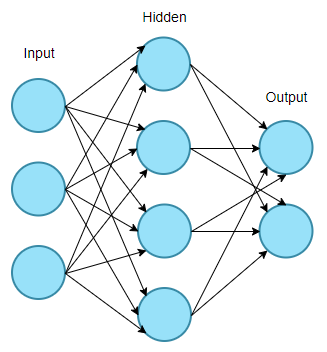
\includegraphics[width=10cm]{figures/1174083/figures7/8.png}
	\caption{gambaran penjelasan no. 9}
\end{figure}

\subsubsection{Jelaskan apa maksud dari fungsi di listing 7.3. dengan parameter tersebut}
\hfill\\
\lstinputlisting[firstline=32, lastline=33, caption={compile model},captionpos=b]{src/1174083/src7/teori.py}
Melakukan peng compile-an dari model Sequential tadi dengan Loss yandengang merupakan fungsi optimisasi skor menggunakan categorical crossentropy , dan menggunakan algoritma adam sebagai optimizer. Adam yaitu algoritma pengoptimalan yang dapat digunakan sebagai ganti dari prosedur penurunan gradien stokastik klasik untuk memperbarui bobot jaringan yang berulang berdasarkan data training.Dengan metrik yaitu fungsi yang digunakan untuk menilai kinerja mode Anda disini menggunakan fungsi accuracy.
\begin{figure}[H]
	\centering
	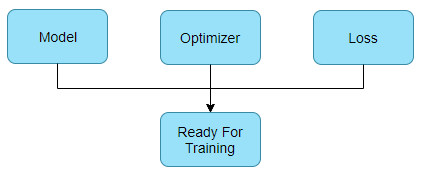
\includegraphics[width=10cm]{figures/1174083/figures7/9.png}
	\caption{gambaran penjelasan no. 9}
\end{figure}

\subsubsection{Jelaskan apa itu Deep Learning}
\hfill\\
Deep Learning adalah subbidang machine learning yang berkaitan dengan algoritma yang terinspirasi oleh struktur dan fungsi otak yang disebut jaringan saraf tiruan atau Artificial Neural Networks. Jaringan saraf tiruan, algoritma yang terinspirasi oleh otak manusia, belajar dari sejumlah besar data. Demikian pula dengan bagaimana kita belajar dari pengalaman, algoritma pembelajaran yang mendalam akan melakukan tugas berulang kali, setiap kali sedikit mengubahnya untuk meningkatkan hasilnya.

\subsubsection{Jelaskan apa itu Deep Neural Network, dan apa bedanya dengan Deep Learning}
\hfill\\
Deep Neural Network adalah jaringan syaraf tiruan (JST) dengan beberapa lapisan antara lapisan input dan output. DNN menemukan manipulasi matematis yang benar untuk mengubah input menjadi output, apakah itu hubungan linear atau hubungan non-linear. Merupakan jaringan syaraf dengan tingkat kompleksitas tertentu, jaringan syaraf dengan lebih dari dua lapisan. Deep Neural Network menggunakan pemodelan matematika yang canggih untuk memproses data dengan cara yang kompleks.

	DNN hanya terdiri dari dua laipsan yaitu input dan output, sedangkan dalam Deep learning kita dapat mendefiniskan layer sebanyak yang kita inginkan atau butuhkan.

\subsubsection{Jelaskan dengan ilustrasi gambar buatan sendiri(langkah per langkah) bagaimana perhitungan algoritma konvolusi dengan ukuran stride (NPM mod 3+1) x (NPM mod 3+1) yang terdapat max pooling} 
\hfill\\
Stride adalah parameter yang menentukan berapa jumlah pergeseran filter.
stride = (NPM mod 3+1) x (NPM mod 3+1) = 1
\begin{itemize}
\item disini saya mempunyai data seperti berikut:
\begin{figure}[H]
	\centering
	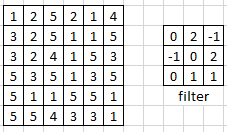
\includegraphics[scale=0.5]{figures/1174083/figures7/10.png}
	\caption{gambaran penjelasan no. 9}
\end{figure}

\item Kemudian hitung konvolusi untuk setiap matriksnya seperti berikut :
	\begin{itemize}
		\item pertama
			\begin{figure}[H]
				\centering
				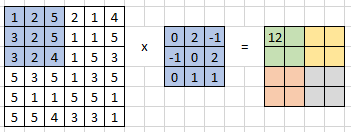
\includegraphics[scale=1]{figures/1174083/figures7/11.png}
				\caption{Algoritma Konvolusi}
			\end{figure}

		\item kedua
			\begin{figure}[H]
				\centering
				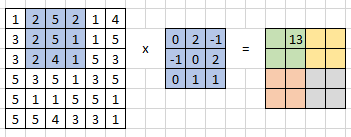
\includegraphics[scale=1]{figures/1174083/figures7/12.png}
				\caption{Algoritma Konvolusi}
			\end{figure}

		\item ketiga
			\begin{figure}[H]
				\centering
				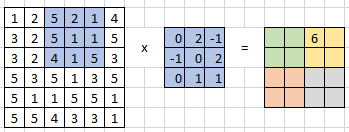
\includegraphics[scale=1]{figures/1174083/figures7/13.png}
				\caption{Algoritma Konvolusi}
			\end{figure}
			
		\item keempat
			\begin{figure}[H]
				\centering
				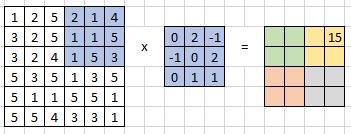
\includegraphics[scale=1]{figures/1174083/figures7/14.png}
				\caption{Algoritma Konvolusi}
			\end{figure}
			
		\item kelima
			\begin{figure}[H]
				\centering
				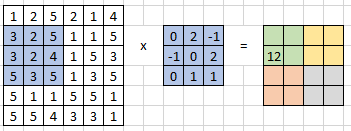
\includegraphics[scale=1]{figures/1174083/figures7/15.png}
				\caption{Algoritma Konvolusi}
			\end{figure}
			
		\item keenam
			\begin{figure}[H]
				\centering
				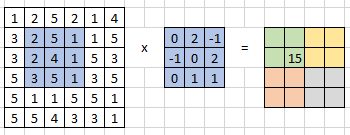
\includegraphics[scale=1]{figures/1174083/figures7/16.png}
				\caption{Algoritma Konvolusi}
			\end{figure}
			
		\item ketujuh
			\begin{figure}[H]
				\centering
				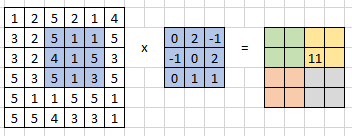
\includegraphics[scale=1]{figures/1174083/figures7/17.png}
				\caption{Algoritma Konvolusi}
			\end{figure}

		\item kedelapan
			\begin{figure}[H]
				\centering
				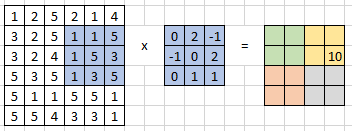
\includegraphics[scale=1]{figures/1174083/figures7/18.png}
				\caption{Algoritma Konvolusi}
			\end{figure}

		\item kesembilan
			\begin{figure}[H]
				\centering
				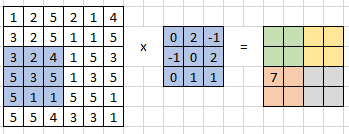
\includegraphics[scale=1]{figures/1174083/figures7/19.png}
				\caption{Algoritma Konvolusi}
			\end{figure}
			
		\item kesepuluh
			\begin{figure}[H]
				\centering
				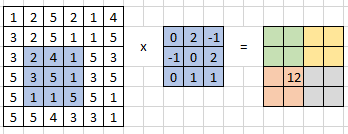
\includegraphics[scale=1]{figures/1174083/figures7/20.png}
				\caption{Algoritma Konvolusi}
			\end{figure}
			
		\item kesebelas
			\begin{figure}[H]
				\centering
				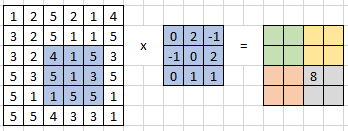
\includegraphics[scale=1]{figures/1174083/figures7/21.png}
				\caption{Algoritma Konvolusi}
			\end{figure}
			
		\item keduabelas
			\begin{figure}[H]
				\centering
				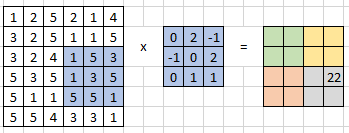
\includegraphics[scale=1]{figures/1174083/figures7/22.png}
				\caption{Algoritma Konvolusi}
			\end{figure}
			
		\item ketigabelas
			\begin{figure}[H]
				\centering
				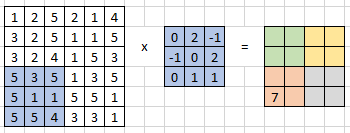
\includegraphics[scale=1]{figures/1174083/figures7/23.png}
				\caption{Algoritma Konvolusi}
			\end{figure}
			
		\item keempatbelas
			\begin{figure}[H]
				\centering
				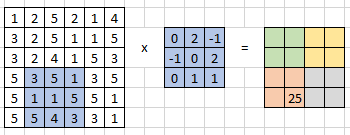
\includegraphics[scale=1]{figures/1174083/figures7/24.png}
				\caption{Algoritma Konvolusi}
			\end{figure}
			
		\item kelimabelas
			\begin{figure}[H]
				\centering
				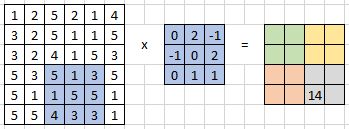
\includegraphics[scale=1]{figures/1174083/figures7/25.png}
				\caption{Algoritma Konvolusi}
			\end{figure}
			
		\item keenambelas
			\begin{figure}[H]
				\centering
				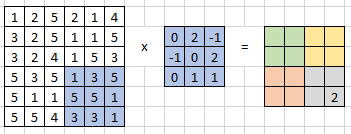
\includegraphics[scale=1]{figures/1174083/figures7/26.png}
				\caption{Algoritma Konvolusi}
			\end{figure}		
	\end{itemize}
	
\item Didapatkan hasil akhir nilai konvolusi dan juga max poolingnya seperti berikut:
\begin{figure}[H]
	\centering
	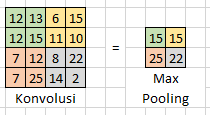
\includegraphics[scale=1]{figures/1174083/figures7/27.png}
	\caption{Hasil akhir nilai konvolusi dan max pooling}
\end{figure}
\end{itemize}

\subsection{Praktek}
\subsubsection{Jelaskan kode program pada blok  In[1]. Jelaskan arti dari setiap baris kode yang dibuat(harus beda dengan teman sekelas) dan hasil luarannya dari komputer sendiri}
\hfill\\
Penjelasan kode:
\lstinputlisting[firstline=8, lastline=11, caption={Kode program blok(1)},captionpos=b]{src/1174083/src7/1174083.py}
Hasil Skrinsut:
\begin{figure}[H]
	\centering
	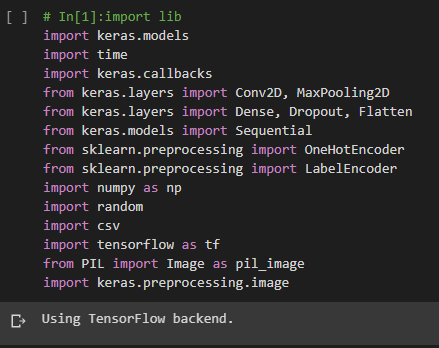
\includegraphics[scale=0.5]{figures/1174083/figures7/p1.png}
	\caption{Hasil Skrinsut}
\end{figure}


\subsubsection{Jelaskan kode program pada blok  In[2]. Jelaskan arti dari setiap baris kode yang dibuat(harus beda dengan teman sekelas) dan hasil luarannya dari komputer sendiri}
\hfill\\
Penjelasan kode:
\lstinputlisting[firstline=13, lastline=27, caption={Kode program blok(2)},captionpos=b]{src/1174083/src7/1174083.py}
Hasil Skrinsut:
\begin{figure}[H]
	\centering
	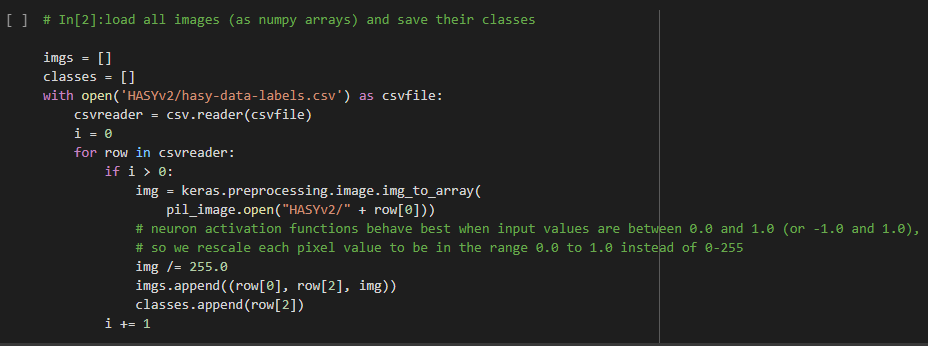
\includegraphics[scale=0.5]{figures/1174083/figures7/p2.png}
	\caption{Hasil Skrinsut}
\end{figure}


\subsubsection{Jelaskan kode program pada blok  In[3]. Jelaskan arti dari setiap baris kode yang dibuat(harus beda dengan teman sekelas) dan hasil luarannya dari komputer sendiri}
\hfill\\
Penjelasan kode:
\lstinputlisting[firstline=29, lastline=34, caption={Kode program blok(3)},captionpos=b]{src/1174083/src7/1174083.py}
Hasil Skrinsut:
\begin{figure}[H]
	\centering
	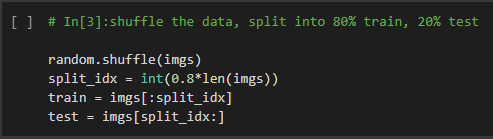
\includegraphics[scale=0.5]{figures/1174083/figures7/p3.png}
	\caption{Hasil Skrinsut}
\end{figure}



\subsubsection{Jelaskan kode program pada blok  In[4]. Jelaskan arti dari setiap baris kode yang dibuat(harus beda dengan teman sekelas) dan hasil luarannya dari komputer sendiri}
\hfill\\
Penjelasan kode:
\lstinputlisting[firstline=36, lastline=41, caption={Kode program blok(4)},captionpos=b]{src/1174083/src7/1174083.py}
Hasil Skrinsut:
\begin{figure}[H]
	\centering
	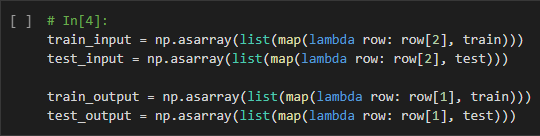
\includegraphics[scale=0.5]{figures/1174083/figures7/p4.png}
	\caption{Hasil Skrinsut}
\end{figure}
	

\subsubsection{Jelaskan kode program pada blok  In[5]. Jelaskan arti dari setiap baris kode yang dibuat(harus beda dengan teman sekelas) dan hasil luarannya dari komputer sendiri}
\hfill\\
Penjelasan kode:
\lstinputlisting[firstline=43, lastline=45, caption={Kode program blok(5)},captionpos=b]{src/1174083/src7/1174083.py}
Hasil Skrinsut:
\begin{figure}[H]
	\centering
	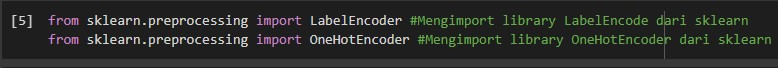
\includegraphics[scale=0.5]{figures/1174083/figures7/p5.png}
	\caption{Hasil Skrinsut}
\end{figure}


\subsubsection{Jelaskan kode program pada blok  In[6]. Jelaskan arti dari setiap baris kode yang dibuat(harus beda dengan teman sekelas) dan hasil luarannya dari komputer sendiri}
\hfill\\
Penjelasan kode:
\lstinputlisting[firstline=47, lastline=49, caption={Kode program blok(6)},captionpos=b]{src/1174083/src7/1174083.py}
Hasil Skrinsut:
\begin{figure}[H]
	\centering
	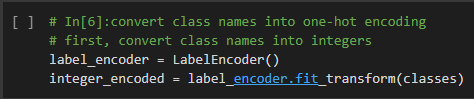
\includegraphics[scale=0.5]{figures/1174083/figures7/p6.png}
	\caption{Hasil Skrinsut}
\end{figure}


\subsubsection{Jelaskan kode program pada blok  In[7]. Jelaskan arti dari setiap baris kode yang dibuat(harus beda dengan teman sekelas) dan hasil luarannya dari komputer sendiri}
\hfill\\
Penjelasan kode:
\lstinputlisting[firstline=36, lastline=41, caption={Kode program blok(7)},captionpos=b]{src/1174083/src7/1174083.py}
Hasil Skrinsut:
\begin{figure}[H]
	\centering
	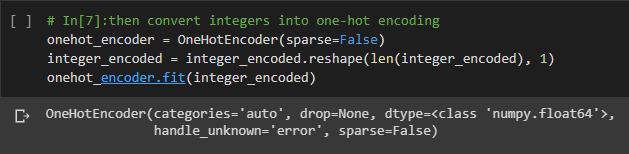
\includegraphics[scale=0.5]{figures/1174083/figures7/p7.png}
	\caption{Hasil Skrinsut}
\end{figure}


\subsubsection{Jelaskan kode program pada blok In[8]. Jelaskan arti dari setiap baris kode yang dibuat(harus beda dengan teman sekelas) dan hasil luarannya dari komputer sendiri}
\hfill\\
Penjelasan kode:
\lstinputlisting[firstline=56, lastline=62, caption={Kode program blok(8)},captionpos=b]{src/1174083/src7/1174083.py}
Hasil Skrinsut:
\begin{figure}[H]
	\centering
	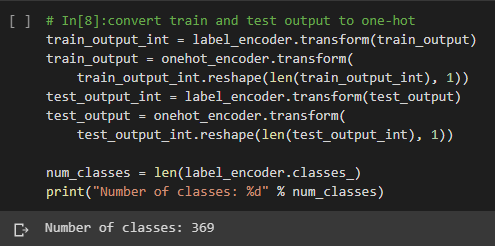
\includegraphics[scale=0.5]{figures/1174083/figures7/p8.png}
	\caption{Hasil Skrinsut}
\end{figure}


\subsubsection{Jelaskan kode program pada blok In[9]. Jelaskan arti dari setiap baris kode yang dibuat(harus beda dengan teman sekelas) dan hasil luarannya dari komputer sendiri}
\hfill\\

Penjelasan kode:
\lstinputlisting[firstline=64, lastline=68, caption={Kode program blok(9)},captionpos=b]{src/1174083/src7/1174083.py}
Hasil Skrinsut:
\begin{figure}[H]
	\centering
	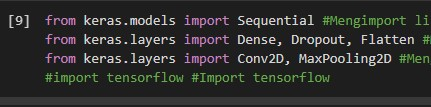
\includegraphics[scale=0.5]{figures/1174083/figures7/p9.png}
	\caption{Hasil Skrinsut}
\end{figure}


\subsubsection{Jelaskan kode program pada blok  In[10]. Jelaskan arti dari setiap baris kode yang dibuat(harus beda dengan teman sekelas) dan hasil luarannya dari komputer sendiri}
\hfill\\
Penjelasan kode:
\lstinputlisting[firstline=70, lastline=83, caption={Kode program blok(10)},captionpos=b]{src/1174083/src7/1174083.py}
Hasil Skrinsut:
\begin{figure}[H]
	\centering
	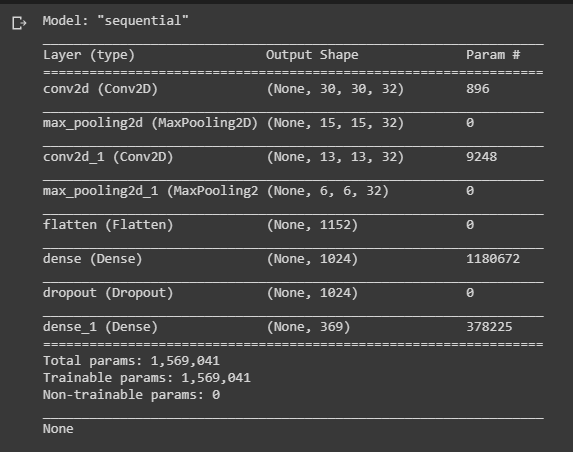
\includegraphics[scale=0.5]{figures/1174083/figures7/p10.png}
	\caption{Hasil Skrinsut}
\end{figure}

\subsubsection{Jelaskan kode program pada blok  In[11]. Jelaskan arti dari setiap baris kode yang dibuat(harus beda dengan teman sekelas) dan hasil luarannya dari komputer sendiri}
\hfill\\
Penjelasan kode:
\lstinputlisting[firstline=85, lastline=87, caption={Kode program blok(11)},captionpos=b]{src/1174083/src7/1174083.py}
Hasil Skrinsut:
\begin{figure}[H]
	\centering
	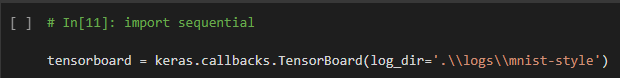
\includegraphics[scale=0.5]{figures/1174083/figures7/p11.png}
	\caption{Hasil Skrinsut}
\end{figure}


\subsubsection{Jelaskan kode program pada blok  In[12]. Jelaskan arti dari setiap baris kode yang dibuat(harus beda dengan teman sekelas) dan hasil luarannya dari komputer sendiri}
\hfill\\
Penjelasan kode:
\lstinputlisting[firstline=89, lastline=99, caption={Kode program blok(12)},captionpos=b]{src/1174083/src7/1174083.py}
Hasil Skrinsut:
\begin{figure}[H]
	\centering
	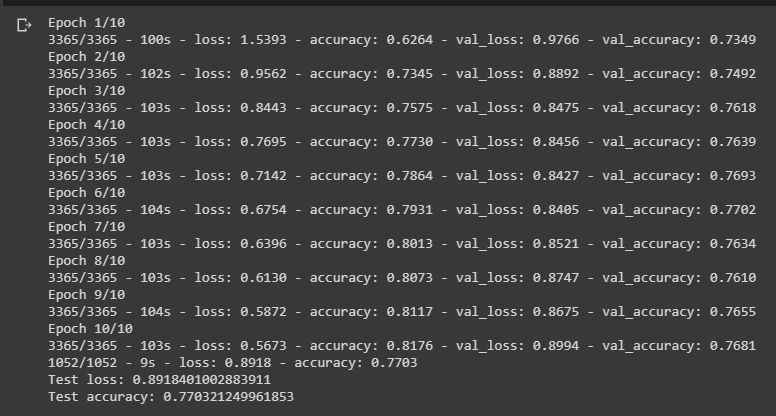
\includegraphics[scale=0.5]{figures/1174083/figures7/p12.png}
	\caption{Hasil Skrinsut}
\end{figure}


\subsubsection{Jelaskan kode program pada blok  In[13]. Jelaskan arti dari setiap baris kode yang dibuat(harus beda dengan teman sekelas) dan hasil luarannya dari komputer sendiri}
\hfill\\
Penjelasan kode:
\lstinputlisting[firstline=101, lastline=130, caption={Kode program blok(13)},captionpos=b]{src/1174083/src7/1174083.py}
Hasil Skrinsut:
\begin{figure}[H]
	\centering
	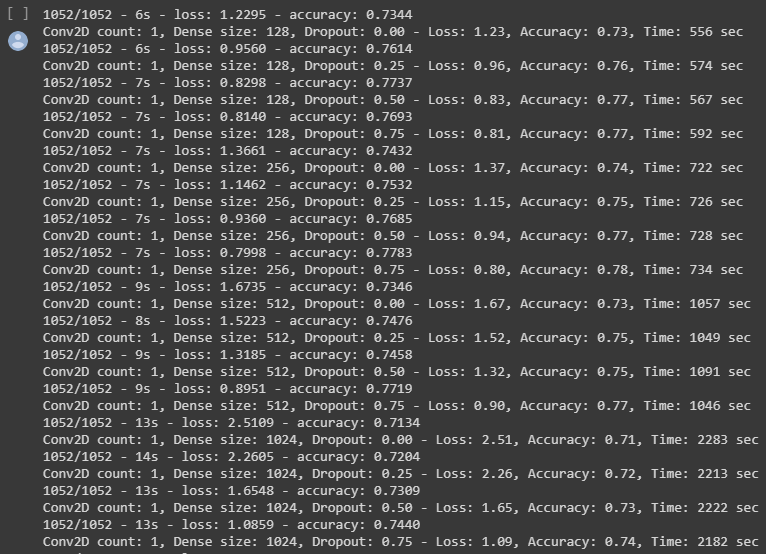
\includegraphics[scale=0.5]{figures/1174083/figures7/p13a.png}
	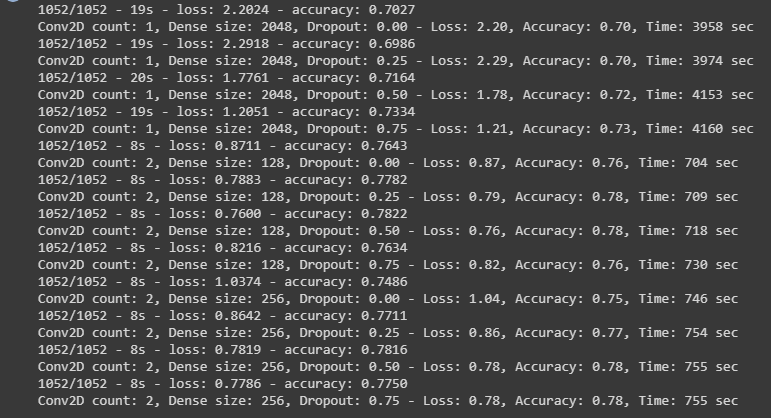
\includegraphics[scale=0.5]{figures/1174083/figures7/p13b.png}
	\caption{Hasil Skrinsut}
\end{figure}


\subsubsection{Jelaskan kode program pada blok  In[14]. Jelaskan arti dari setiap baris kode yang dibuat(harus beda dengan teman sekelas) dan hasil luarannya dari komputer sendiri}
\hfill\\
Penjelasan kode:
\lstinputlisting[firstline=132, lastline=143, caption={Kode program blok(14)},captionpos=b]{src/1174083/src7/1174083.py}
Hasil Skrinsut:
\begin{figure}[H]
	\centering
	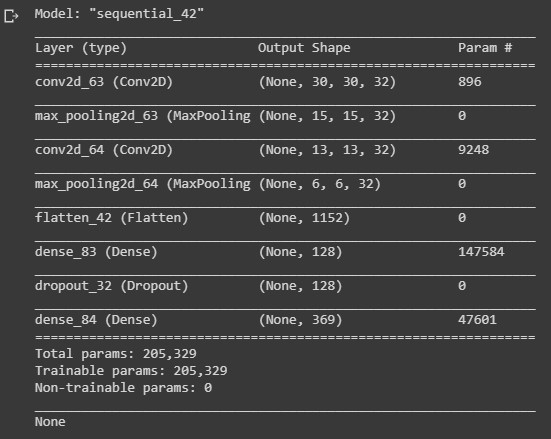
\includegraphics[scale=0.5]{figures/1174083/figures7/p14.png}
	\caption{Hasil Skrinsut}
\end{figure}

\subsubsection{Jelaskan kode program pada blok  In[15]. Jelaskan arti dari setiap baris kode yang dibuat(harus beda dengan teman sekelas) dan hasil luarannya dari komputer sendiri}
\hfill\\
Penjelasan kode:
\lstinputlisting[firstline=145, lastline=148, caption={Kode program blok(15)},captionpos=b]{src/1174083/src7/1174083.py}
Hasil Skrinsut:
\begin{figure}[H]
	\centering
	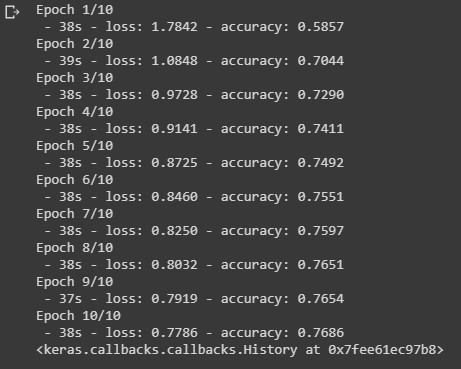
\includegraphics[scale=0.5]{figures/1174083/figures7/p15.png}
	\caption{Hasil Skrinsut}
\end{figure}


\subsubsection{Jelaskan kode program pada blok  In[16]. Jelaskan arti dari setiap baris kode yang dibuat(harus beda dengan teman sekelas) dan hasil luarannya dari komputer sendiri}
\hfill\\
Penjelasan kode:
\lstinputlisting[firstline=150, lastline=151, caption={Kode program blok(16)},captionpos=b]{src/1174083/src7/1174083.py}
Hasil Skrinsut:
\begin{figure}[H]
	\centering
	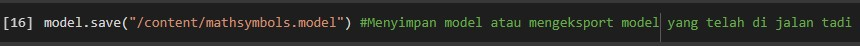
\includegraphics[scale=0.5]{figures/1174083/figures7/p16.png}
	\caption{Hasil Skrinsut}
\end{figure}


\subsubsection{Jelaskan kode program pada blok  In[17]. Jelaskan arti dari setiap baris kode yang dibuat(harus beda dengan teman sekelas) dan hasil luarannya dari komputer sendiri}
\hfill\\
Penjelasan kode:
\lstinputlisting[firstline=153, lastline=154, caption={Kode program blok(17)},captionpos=b]{src/1174083/src7/1174083.py}
Hasil Skrinsut:
\begin{figure}[H]
	\centering
	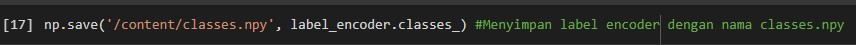
\includegraphics[scale=0.5]{figures/1174083/figures7/p17.png}
	\caption{Hasil Skrinsut}
\end{figure}


\subsubsection{Jelaskan kode program pada blok In[18]. Jelaskan arti dari setiap baris kode yang dibuat(harus beda dengan teman sekelas) dan hasil luarannya dari komputer sendiri}
\hfill\\Penjelasan kode:
\lstinputlisting[firstline=156, lastline=160, caption={Kode program blok(18)},captionpos=b]{src/1174083/src7/1174083.py}
Hasil Skrinsut:
\begin{figure}[H]
	\centering
	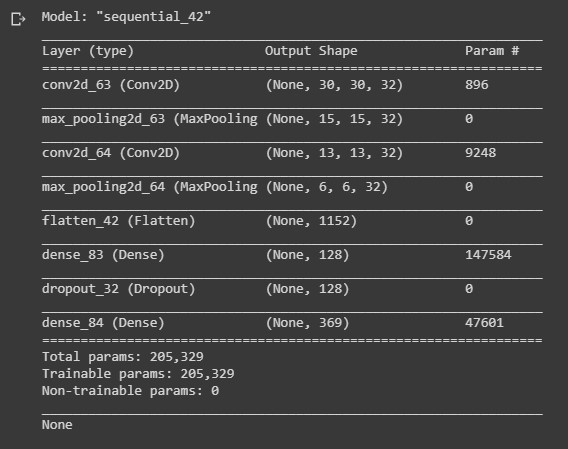
\includegraphics[scale=0.5]{figures/1174083/figures7/p18.png}
	\caption{Hasil Skrinsut}
\end{figure}


\subsubsection{Jelaskan kode program pada blok  In[19]. Jelaskan arti dari setiap baris kode yang dibuat(harus beda dengan teman sekelas) dan hasil luarannya dari komputer sendiri}
\hfill\\Penjelasan kode:
\lstinputlisting[firstline=162, lastline=174, caption={Kode program blok(19)},captionpos=b]{src/1174083/src7/1174083.py}
Hasil Skrinsut:
\begin{figure}[H]
	\centering
	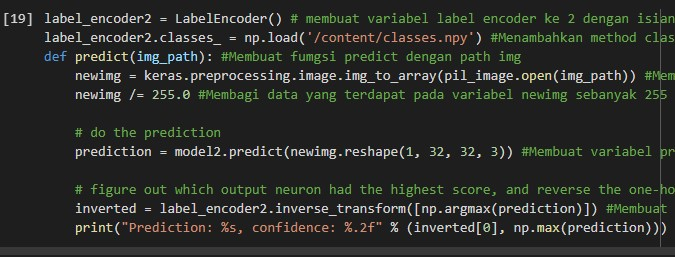
\includegraphics[scale=0.5]{figures/1174083/figures7/p19.png}
	\caption{Hasil Skrinsut}
\end{figure}


\subsubsection{Jelaskan kode program pada blok  In[20]. Jelaskan arti dari setiap baris kode yang dibuat(harus beda dengan teman sekelas) dan hasil luarannya dari komputer sendiri}
\hfill\\
Penjelasan kode:
\lstinputlisting[firstline=176, lastline=179, caption={Kode program blok(20)},captionpos=b]{src/1174083/src7/1174083.py}
Hasil Skrinsut:
\begin{figure}[H]
	\centering
	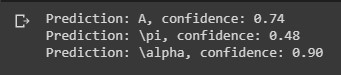
\includegraphics[scale=0.5]{figures/1174083/figures7/p20.png}
	\caption{Hasil Skrinsut}
\end{figure}

\subsection{Penanganan Error}
\subsubsection{Terjadi error}
\hfill\\
\begin{enumerate}
\item terjadi error invalid argument, seperti pada gambar berikut:
\begin{figure}[H]
	\centering
	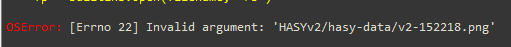
\includegraphics[width=8cm]{figures/1174083/figures7/error1.png}
	\caption{terjadi Error 1}
\end{figure}

\item terjadi error Sequential has no attribute, seperti pada gambar berikut:
\begin{figure}[H]
	\centering
	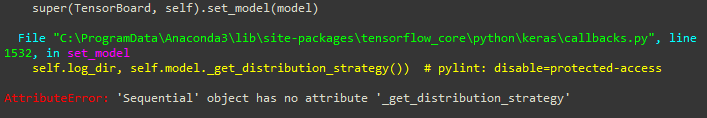
\includegraphics[width=8cm]{figures/1174083/figures7/error2.png}
	\caption{terjadi Error 2}
\end{figure}
\end{enumerate}

\subsubsection{Solusi}
\hfill\\
\begin{enumerate}
\item solusi dari error 1 ialah:
membenarkan argumen, karena terdapat typo

\item solusi dari error 2 ialah:
proses running yang tidak sempurna pada blok sebelumnya, sehingga harus dijalan kan lagi dengan benar.

\end{enumerate}

\subsection{Bukti Tidak Plagiat}
\begin{figure}[H]
	\centering
	\includegraphics[width=12cm]{figures/1174083/figures7/plagiarism.png}
	\caption{Bukti tidak plagiat}
\end{figure}

\subsection{Link Youtube}
https://bit.ly/baktiListVideo